\documentclass[14pt]{matmex-diploma-custom}
\usepackage{enumitem}
\usepackage{amsmath}

% * <svitkovsergey@gmail.com> 13:38:37 13 Dec 2016 UTC+0300:
% ping
\begin{document}
\filltitle{ru}{
    chair              = {Кафедра Системного программирования},
    title              = {Реализация поиска путей с КС-ограничениями в рамках библиотеки YC.QuickGraph},
    type               = {coursework},
    position           = {студента},
    group              = 344,
    author             = {Свитков Сергей Андреевич},
    supervisorPosition = {ст. преп, к. ф-м. н.},
    supervisor         = {Григорьев С.\,В.},
}
\maketitle
\tableofcontents
%\section*{Аннотация}
%	Большинство промышленных языков для написания запросов к графовым базам данных являются регулярными. Но регулярные языки не применимы в ряде задач, поэтому актуальным является создание контекстно-свободного (далее --- КС) языка запросов. Существуют работы по этой теме, но они в основном теоретические. В данной работе рассматривается практическая реализация механизма контекстно-свободных запросов к ориентированным графам с помеченными ребрами для платформы .NET. Результатом работы является библиотека, предоставляющая набор функций для написания КС-запросов к графам. Полученные результаты могут быть применены в проектах, использующих C\# или F\#.

\section*{Введение}
	Модель представления данных в виде ориентированных графов с метками на ребрах имеет широкую область применения и используется в биоинформатике, социальных исследованиях (например, при представлении социальных графов), semantic web, при реализации графовых баз данных. 
	
	При наличии данных, представленных в виде такой структуры, возникает задача их обработки. Наиболее часто требуется выбрать из всего набора данных какую-либо конкретную часть. Такие задачи в базах данных решаются, как правило, с помощью задания запросов на некоем специализированном языке. Существует множество таких языков, применительно к графовым базам данных наиболее известными являются Gremlin\cite{Gremlin}, Cypher\cite{Cypher}, используемые в графовых базах данных Titan и Neo4J соответственно. Однако, эти языки являются регулярными, а значит, не могут применяться для решения ряда задач. Например, при разборе генеалогического дерева часто возникает задача поиска потомков общего предка. Она решается поиском строк вида \(parent^nchild^n\). Но такие строки не могут содержаться в регулярных языках, однако, существуют в языке, задаваемом контекстно-свободной (в дальнейшем --- КС) грамматикой с правилами вывода \(N \to parent\,child, \,N \to parentN\, child\). Таким образом, актуальной задачей является применение КС-языков запросов для расширения класса задач, решаемых с помощью регулярных языков. 
	
	Существуют работы, предлагающие различные подходы к реализации языков запросов, например \cite{sevon2008subgraph}, \cite{hellings2014conjunctive}, \cite{zhang2016context}, \cite{abiteboul1997regular}, \cite{koschmieder2012regular}. Большая часть из них представляет только теоретические сведения о реализации, а те, что реализованы на практике, имеют довольно ограниченный функционал или же очень узкую специализацию. Однако, как уже было отмечено ранее, класс задач, решение которых возможно с помощью КС-запросов, является обширным. Исходя из этого, реализация средства для выполнения запросов должна быть применима для решения различных задач, связанных с данной тематикой. Логично, что для соответствия этим требованиям необходим широкий функционал и различные форматы представления результата запроса. Из этого можно сделать вывод о том, что для возможности применить реализацию к различным задачам обработки графовых структур данных, её удобнее всего оформить как библиотеку. Исходя из этого было принято решение реализовать библиотеку для выполнения КС-запросов к графам, позволяющую представить результат исполнения запроса в нескольких форматах.
	
	В качестве платформы для реализации была выбрана .NET. Для неё существует ряд библиотек для работы с графами, например GraphSharp \cite{graphsharp}, Automatic Graph Layout \cite{agl}, но наиболее известной является QuickGraph \cite{quickgraph}, работа над которой прекращена в 2011 году. В лаборатории языковых инструментов JetBrains с 2015 года ведется разработка и поддержка библиотеки YC.QuickGraph \cite{YC.QuickGraph}, за основу которой была взята QuickGraph. В данной библиотеке имеется множество инструментов для работы с графами, поэтому было принято решение использовать её для реализации. В качестве алгоритма для синтаксического анализа графов используется GLL\cite{gll}, поскольку он имеет хорошую асимптотику и может обрабатывать все КС-грамматики, в том числе и лево-рекурсивные, а так же в рамках работы \cite{ragRelaxedParsing} был реализован и интегрирован в YaccConstructor \cite{YaccConstructorPage}, \cite{авдюхин2012создание}, \cite{кириленко2013разработка}, \cite{gsv_phd}, \cite{кириленко2013разработка}, \cite{азимов2016syntax}, \cite{ковалев2016реализация}, \cite{полубелова2014генератор} --- исследовательский проект лаборатории языковых инструментов JetBrains, представляющий собой набор инструментов для решения различных задач синтаксического и лексического анализа, реализованный для платформы .NET.
	
\section{Постановка задачи}
    Резюмируя сказанное во введении, была поставлена цель работы: реализовать библиотеку для выполнения КС-запросов к графам, используя .NET как основную платформу, YC.QuickGraph --- в качестве библиотеки для представления графов и YaccConstructor в качестве набора инструментов для решения задач синтаксического анализа. Результат работы позволяет выполнять КС-запросы к ориентированным графам с помеченными ребрами и представлять результат в виде подграфа, множества путей, кратчайшего пути, КС-отношения (\(R = (N,\, n,\, m)\), где \(N\) --- нетерминал, из которого выводим путь из вершины \(n\) в \(m\). ). 
    
    Для достижения данной цели необходимо решить следующие задачи:
	\begin{itemize}
	    \item разработать алгоритм исполнения запроса с КС-ограничениями;
	    \item спроектировать удобный для пользователя интерфейс;
        \item реализовать расширение библиотеки YC.QuickGraph;
        \item опубликовать результат в виде NuGet-пакета.
	\end{itemize}

\section{Обзор предметной области}
	\subsection{Related works}
	В этой секции будут рассмотрены работы, посвященные реализации инструментов для исполнения запросов.
		\subsubsection*{Conjunctive Context-Free Path Queries}
		В данной работе рассматривается построение обобщения существующего регулярного языка запросов к графам с помеченными ребрами CRPQ до КС-языка CCFPQ. Расширение позволяет использовать КС-грамматики вместо регулярных выражений для поиска путей в графе. Предлагаемый в статье алгоритм использует CYK для синтаксического анализа графов. Результатом исполнения запроса является КС-отношение \(R\). К минусам данной работы можно отнести отсутствие практической реализации и возможность представления результата запроса лишь в одном формате.
		\subsubsection*{Subgraph Queries by Context-free Grammars}
		Данная работа рассматривает вопрос о применении КС-запросов в различных задачах биоинформатики. Предложенный в статье подход подразумевает поиск связного подграфа, порождаемого множеством путей, строки из меток на которых выводимы из задаваемой в качестве запроса КС-грамматики. Для синтаксического анализа используется Earley parser \cite{hale2001probabilistic}. Авторами было проведено тестирование алгоритма, предлагаемого в статье, как на случайно сгенерированных, так и на реальных данных. Эксперименты проводились на компьютере с 1GB оперативной памяти, в качестве ОС использовался Linux. Графы, на которых проводилось тестирование алгоритма, генерировались со следующими ограничениями: фиксированный размер в 10000 вершин, изменяемое ограничение на максимальную длину пути, а так же регулируемая вероятность существования ребра между двумя вершинами. Например, запрос к сгенерированному графу с максимальной длиной пути в 9 вершин выполняется около 200 секунд. Эксперименты, поставленные на реальных данных, показали, что для графа с максимальной длиной пути, равной 8 вершинам, время работы алгоритма может достигать 250 секунд. Единственный формат представления результата, а также большое время исполнения запроса являются основными причинами, по которым результаты данной работы едва ли применимы на практике.
		\subsubsection*{Ослабленный синтаксический анализ динамически формируемых выражений на основе алгоритма GLL}
		Работа Анастасии Рагозиной, написанная на кафедре СП Математико-Механического факультета СПбГУ предлагает алгоритм для синтаксического анализа динамически формируемого кода на основе алгоритма GLL, позволяющий проверять выводимость последовательсти меток на ребрах графа в задаваемой грамматике. Предложенный в работе алгоритм позволяет обрабатывать входные данные большого размера и может быть использован, например, при поиске подпоследовательностей в метагеномных сборках. Так же была доказана корректность и завершаемость алгоритма. Следует отметить, что результатом работы алгоритма является лес разбора, представляемый в виде SPPF\cite{SPPF}, который можно отобразить в нужный формат вывода. Учитывая наличие реализации алгоритма для платформы .NET в проекте YaccConstructor, было принято решение использовать результаты этой работы при реализации.

	\subsection{YaccConstructor}
	    YaccConstructor --- исследовательский проект лаборатории языковых инструментов JetBrains, применимый для исследования и решения различных задач синтаксического и лексического анализа. Проект имеет одноименный инструмент с открытыми исходниками, который включает в себя большое количество компонентов, таких, как язык спецификаций грамматик YARD, алгоритмы для преобразования грамматик, алгоритмы для синтаксического анализа графов и др. Большая часть компонент проекта YaccConstructor реализована для платформы .NET на языке F\#. Поскольку проект имеет модульную архитектуру (рис.\ref{arch}), его компоненты могут быть использованы независимо.
	    
        \begin{figure*}
            \centering
            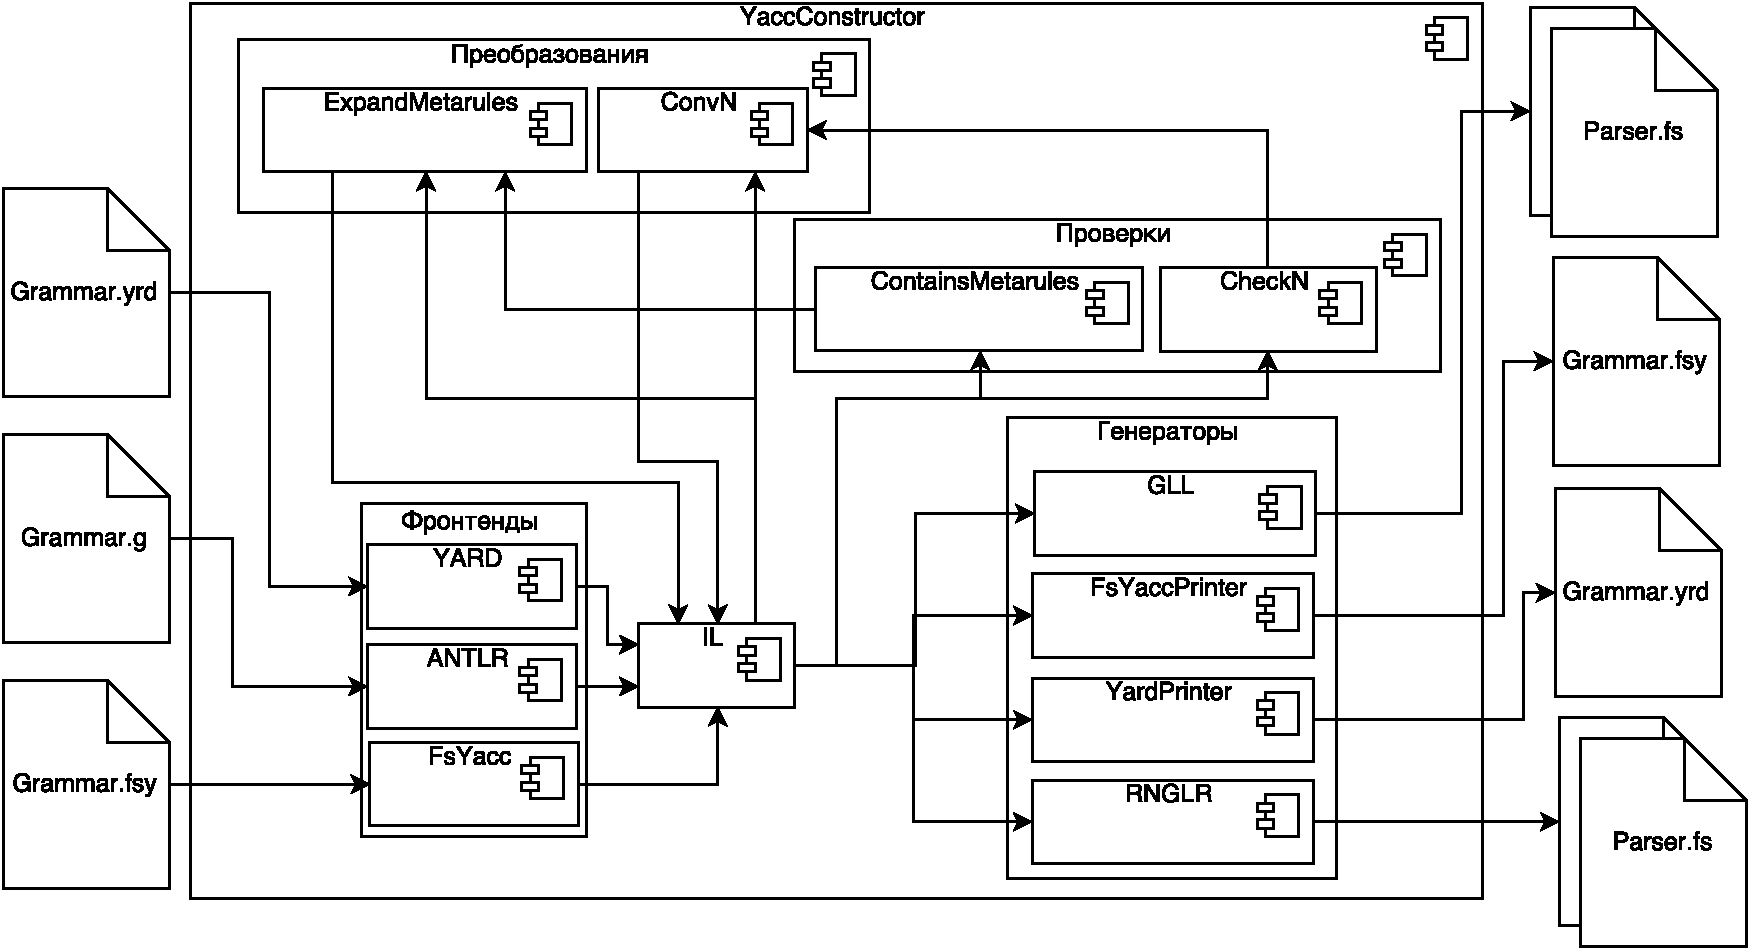
\includegraphics[width=\textwidth]{pics/YCArch.pdf}
            \caption{Архитектура проекта YaccConstructor, заимствована из работы \cite{gsv_phd} \label{arch}}
        \end{figure*}
	    
	    Более подробно рассмотрим такие средства YaccConstructor, как YARD, GLLParser и GLLGenerator. YARD --- язык спецификаций грамматик, позволяющий задавать различные типы грамматик (атрибутные, в нормальной форме Бэкуса-Наура, КС и др.). Так как в рамках данной работы грамматика является запросом, то для его задания будем использовать YARD. GLL --- алгоритм синтаксического анализа, поддерживающий все типы КС-грамматик (в том числе и лево-рекурсивные), кроме того, имеющий асимптотику \(O(n)\) для однозначных граматик и \(O(n^3)\) в худшем случае. В данной работе GLL будет использоваться для синтаксического анализа графов. YaccConstructor имеет 2 модуля, использующих GLL --- GLLGenerator и GLLParser. Первый отвечает за генерацию парсеров для заданных грамматик, а второй, соответственно, за синтаксический анализ. Результатом работы GLLParser является лес разбора --- SPPF, из которого с помощью различных функций, которые планируется реализовать в рамках данной работы, можно получить результат разбора в нужном формате: в виде КС-отношения, подграфа, множества путей или кратчайшего пути.
	\subsection{YC.QuickGraph}
	    YC.QuickGraph --- проект лаборатории языковых инструментов JetBrains, представляющий собой библиотеку для работы с графами на платформе .NET. YC.QuickGraph не является разработанным с нуля проектом, за его основу взята библиотека QuickGraph \cite{quickgraph}, работа над которой была прекращена в 2011 году. YC.QuickGraph имеет средства для представления графов, различные алгоритмы для них (DFS, BFS, поиск кратчайшего пути и др.). Функионал данной библиотеки планируется использовать для представления графа и построения нужного формата вывода.
\section{Реализация}

    \subsection{Архитектура решения}
    
    \begin{figure*}
        \centering
        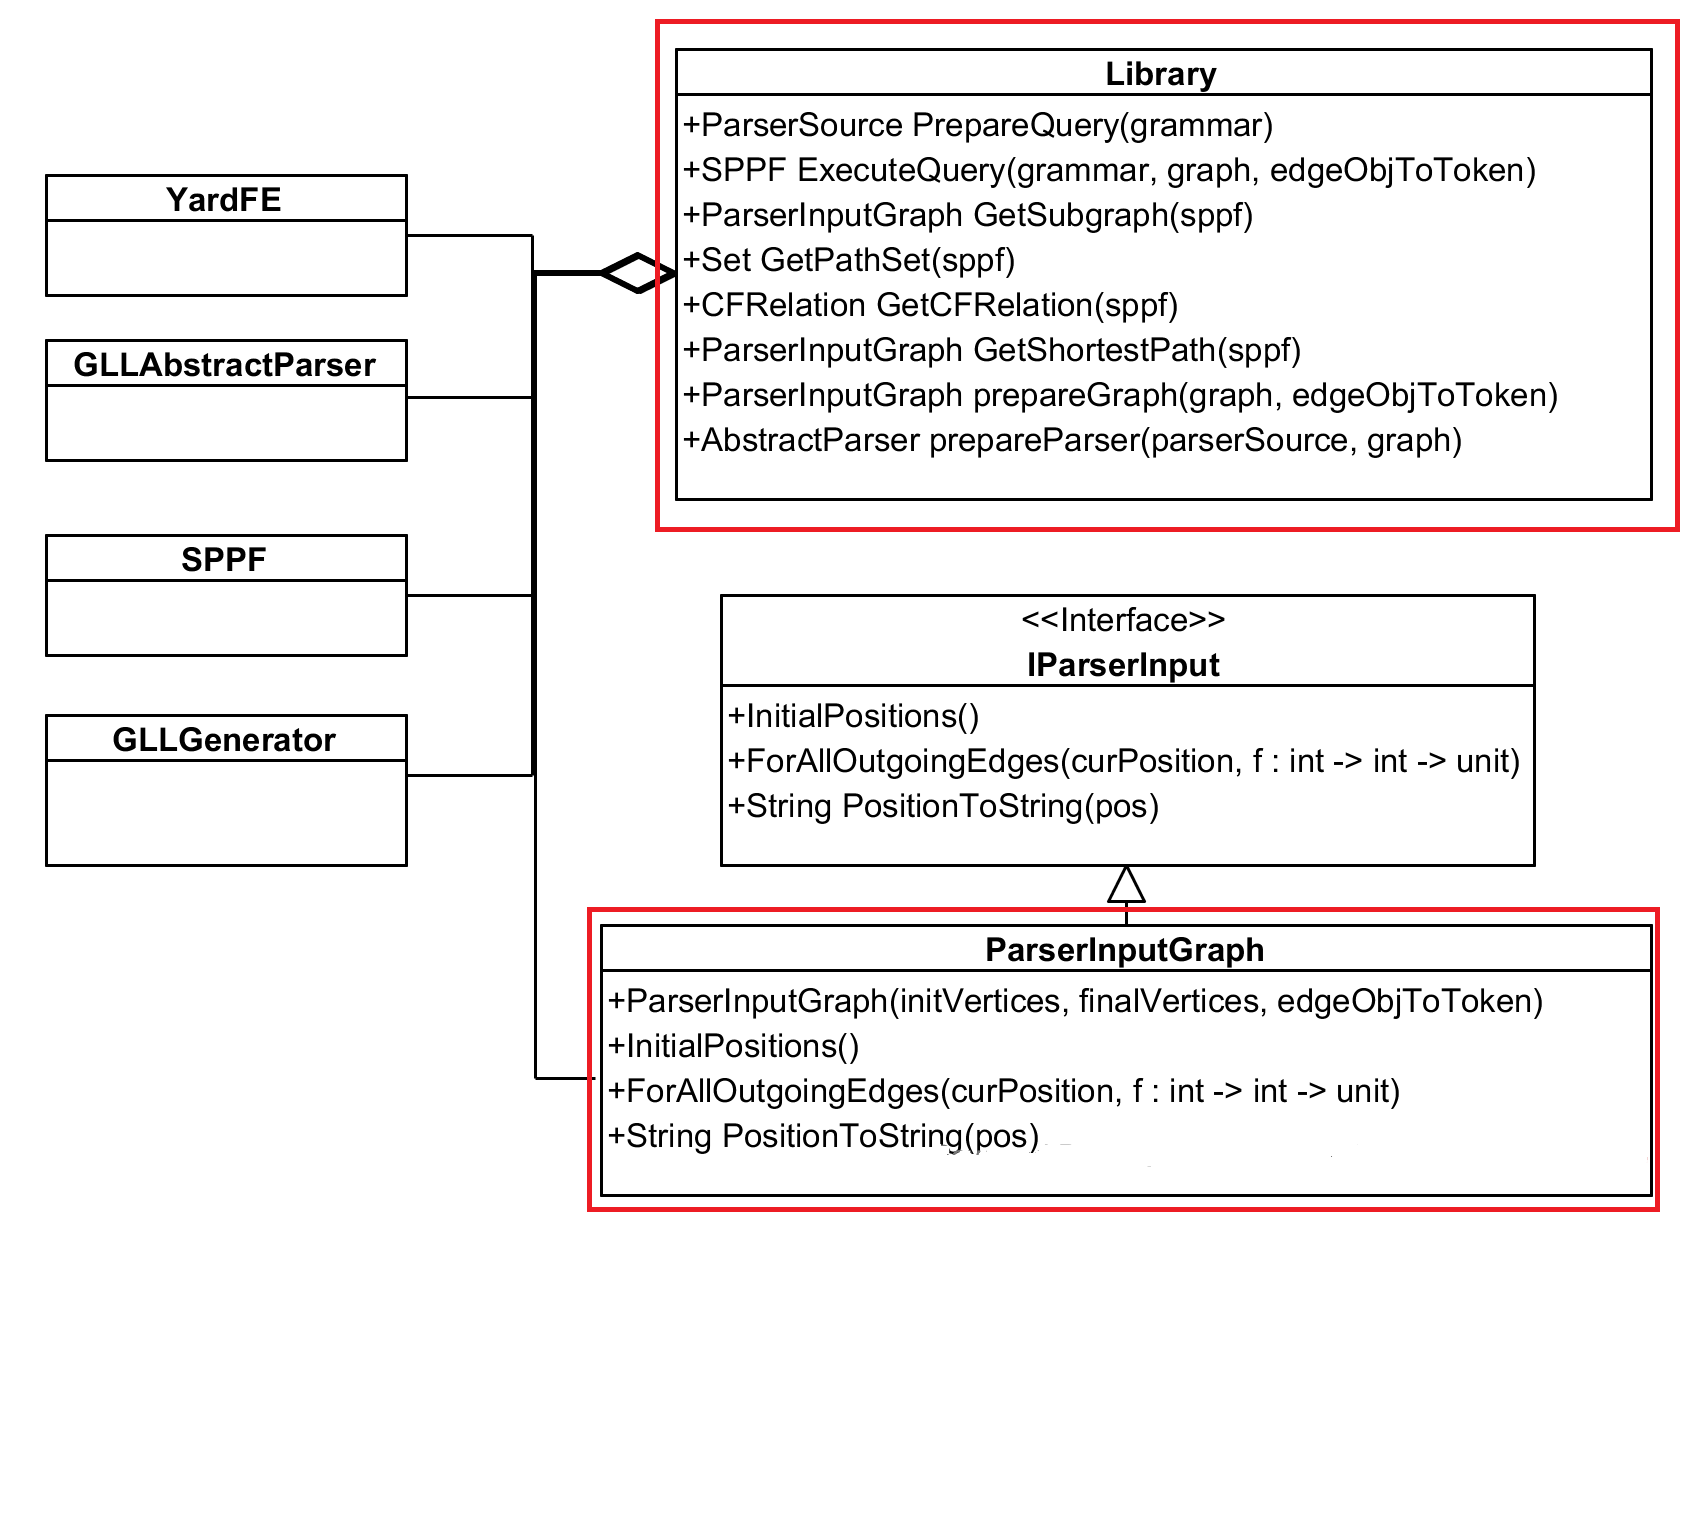
\includegraphics[width=\textwidth]{pics/query.png}
        \caption{Архитектура библиотеки \label{arch_lib}}
    \end{figure*}
    Для предоставления конечному пользователю возможности написания запросов к графу \(G\) и представления результата в одной из нескольких форм была спроектирована архитектура библиотеки (рис.\ref{arch_lib}). При разработке архитектуры были изучены статьи \cite{funcdes1}, \cite{funcdes2}, описывающие основные принципы дизайна функциональных библиотек.
    \begin{figure*}
        \centering
        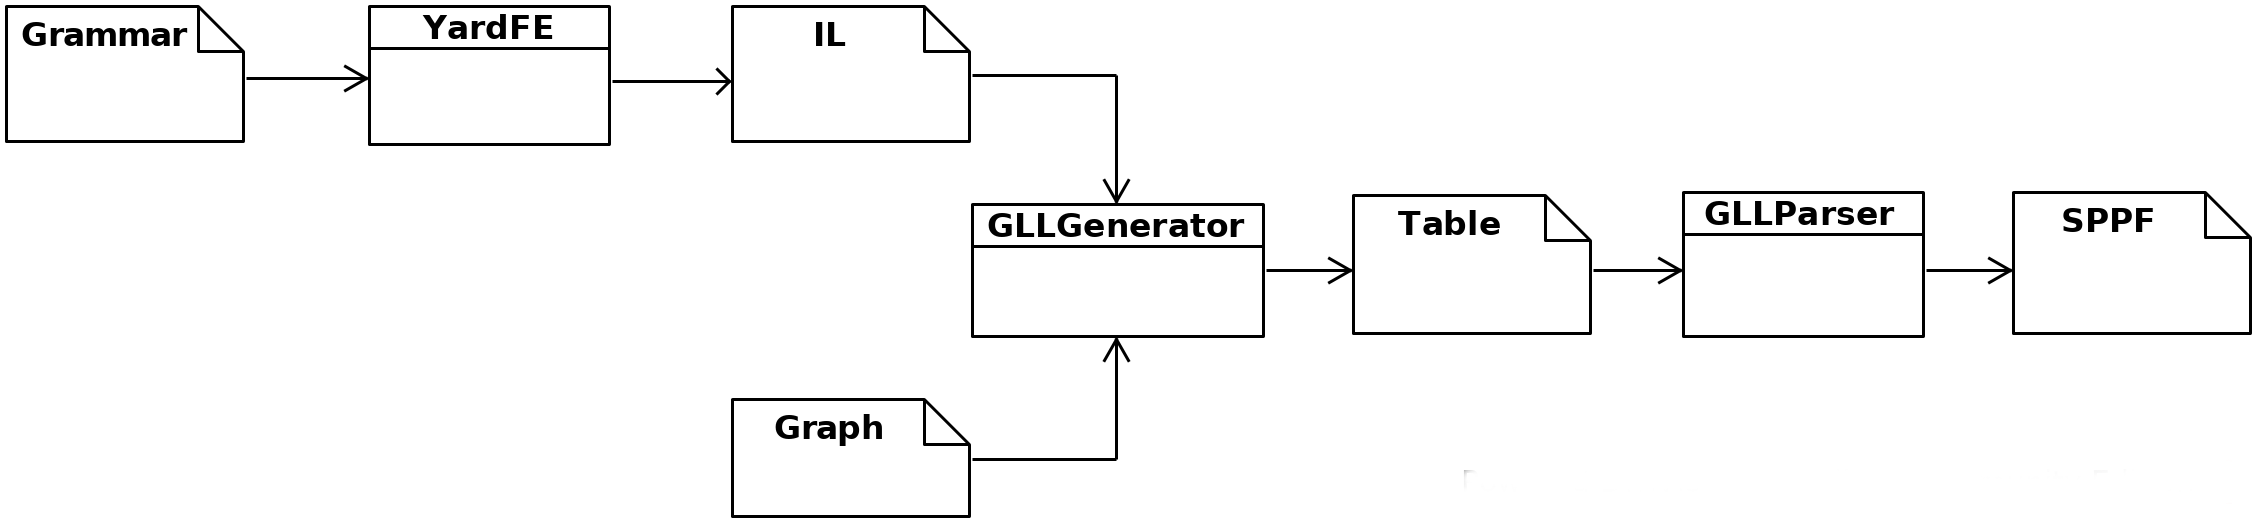
\includegraphics[width=\textwidth]{pics/pipeline.png}
        \caption{Последовательность исполнения запроса \label{pipeline}}
    \end{figure*}
    Пользователь получает возможность написания КС-запросов к задаваемым графам, но само исполнение запроса от него инкапсулировано и производится средствами YaccConstructor и YC.QuickGraph. Существование функций с низким уровнем абстракции позволяет, например, подготовить грамматику для исполнения запроса к нескольким графам. Существование же функций с высоким уровнем абстракции позволит пользователю просто задать запрос к графу и получить результат в желаемом формате. Таким образом, пользователь может комбинировать функции библиотеки, получая инструмент, применимый для решения множества задач.
    
    \subsection{Реализация библиотеки}
    Для реализации библиотеки необходимо было решить ряд инженерных задач задач:
    \begin{itemize}
        \item реализовать класс представления графа, позволяющий преобразовывать пользовательские объекты на рёбрах в токены;
        \item провести рефакторинг модуля, отвечающего за генерацию ParserSourceGLL
        \item добавить поддержку генерации ParserSourceGLL для грамматик, заданных в виде строк;
        \item реализовать преобразования SPPF к подграфу, множеству путей, кратчайшему пути и КС-отношению.
    \end{itemize}
    
    Реализация поддержки преобразования пользовательских объектов на рёбрах графа нужна для запуска алгоритма синтаксического анализа на данном графе, поскольку алгоритм может разбирать только графы с токенами --- численным значениями --- на рёбрах. Сам процесс преобразования объекта инкапсулирован от пользователя; ему достаточно задать граф в виде одной из реализаций, существующих в библиотеке YC.QuickGraph и функцию, преобразующую объект на ребре в строку. После этого заданный граф преобразуется к нужному формату, а функция \(f: EdgeObject -> token\) получается путём комбинации заданной пользователем функции \(g: EdgeObject -> string\) и функции \(u: string -> token\), получаемой из ParserSourceGLL после разбора грамматики с помощью GLLGenerator. После этого на полученном графе и полученном из грамматики ParserSourceGLL можно запустить алгоритм синтаксического анализа.
    
    Модуль, в котором было реализовано преобразование грамматики к ParserSourceGLL, был подвергнут рефакторингу, поскольку ... В связи с этим основная функция, выполняющая преобразование грамматики, была разбита на набор функций с более низким уровнем абстракции, что улучшило читаемость и понятность кода и позволило сохранить изначальную функциональность за счёт комбинации полученных функций. Кроме того, была добавлена поддержка генерации ParserSourceGLL из грамматик, заданных строками.
    
    
\section{Заключение}
В ходе работы достигнуты следующие результаты:
\begin{itemize}
    \item изучена предметная область;
    \item проведен обзор статей, связанных с темой работы;
    \item разработана архитектура (рис.\ref{arch_lib}) предлагаемого решения;
    \item реализована библиотека для выполнения КС-запросов к графам;
    \item написаны тесты и документация.
\end{itemize}
%\section{Основная часть}
%1
%\section{Эксперименты}
%1
\setmonofont[Mapping=tex-text]{CMU Typewriter Text}
\bibliographystyle{ugost2008ls}
\bibliography{coursework}
\end{document}